% results.tex
\chapter{Results}

\section*{Genome Interaction Scaling}
We mapped the reads to the genome as described in the Methods.  Upon mapping reads to interaction matrices, we noted that the number
of observed interactions per bin scales differently by chromosome.  We plotted the percentage of reads observed for each chromosome
in 1Mb bins~\ref{fig:probeScalesMb} and by percentage of chromosome length~\ref{fig:probeScalesPercent}.

\begin{figure}[thp]
  \caption{Chromosome Contacts by Bin}
  \begin{minipage}{0.45\textwidth}%
    \centering
    \caption{}\label{fig:probeScalesMb}
    \includegraphics[width=\textwidth]{./figures/results/probeScalesMb.png}
  \end{minipage}

  \begin{minipage}{0.45\textwidth}
    \centering
    \caption{Contacts by Percent Distance}\label{fig:probeScalesPercent}
    \includegraphics[width=\textwidth]{./figures/results/probeScalesPercent.png}
  \end{minipage}
\end{figure}

% TODO: remark on trans interactions

%We remarked that chromosomes have heterogenous scaling properties.  We examined the character of the chromosome for all replicates
%by computing the x coordinate at which we observed $50\%$ of the total chromosome contacts.  These finding are shown below~\ref{fig:probeCom}.
%
%\begin{figure}
%\end{figure}

\section*{Principal Components and Gene Expression}

We tested whether a change in the compartment character (measured by the principal component) for genomic regions .  Using replicated
IMR90 and hESC gene expression experiments, we plotted the changes in gene expression against the compartment changes, but did not
find any correlation between changes in compartment character and gene expression levels ($\rho = -0.009$, $p$-value negligible.
See Figure~\ref{fig:expressionChangeByCompartment}.)

\begin{figure}[thp]
  \begin{minipage}{0.45\textwidth}%
    \centering
    \caption{Gene Expression Change by Compartment Change}\label{fig:expressionChangeByCompartmentChange}
    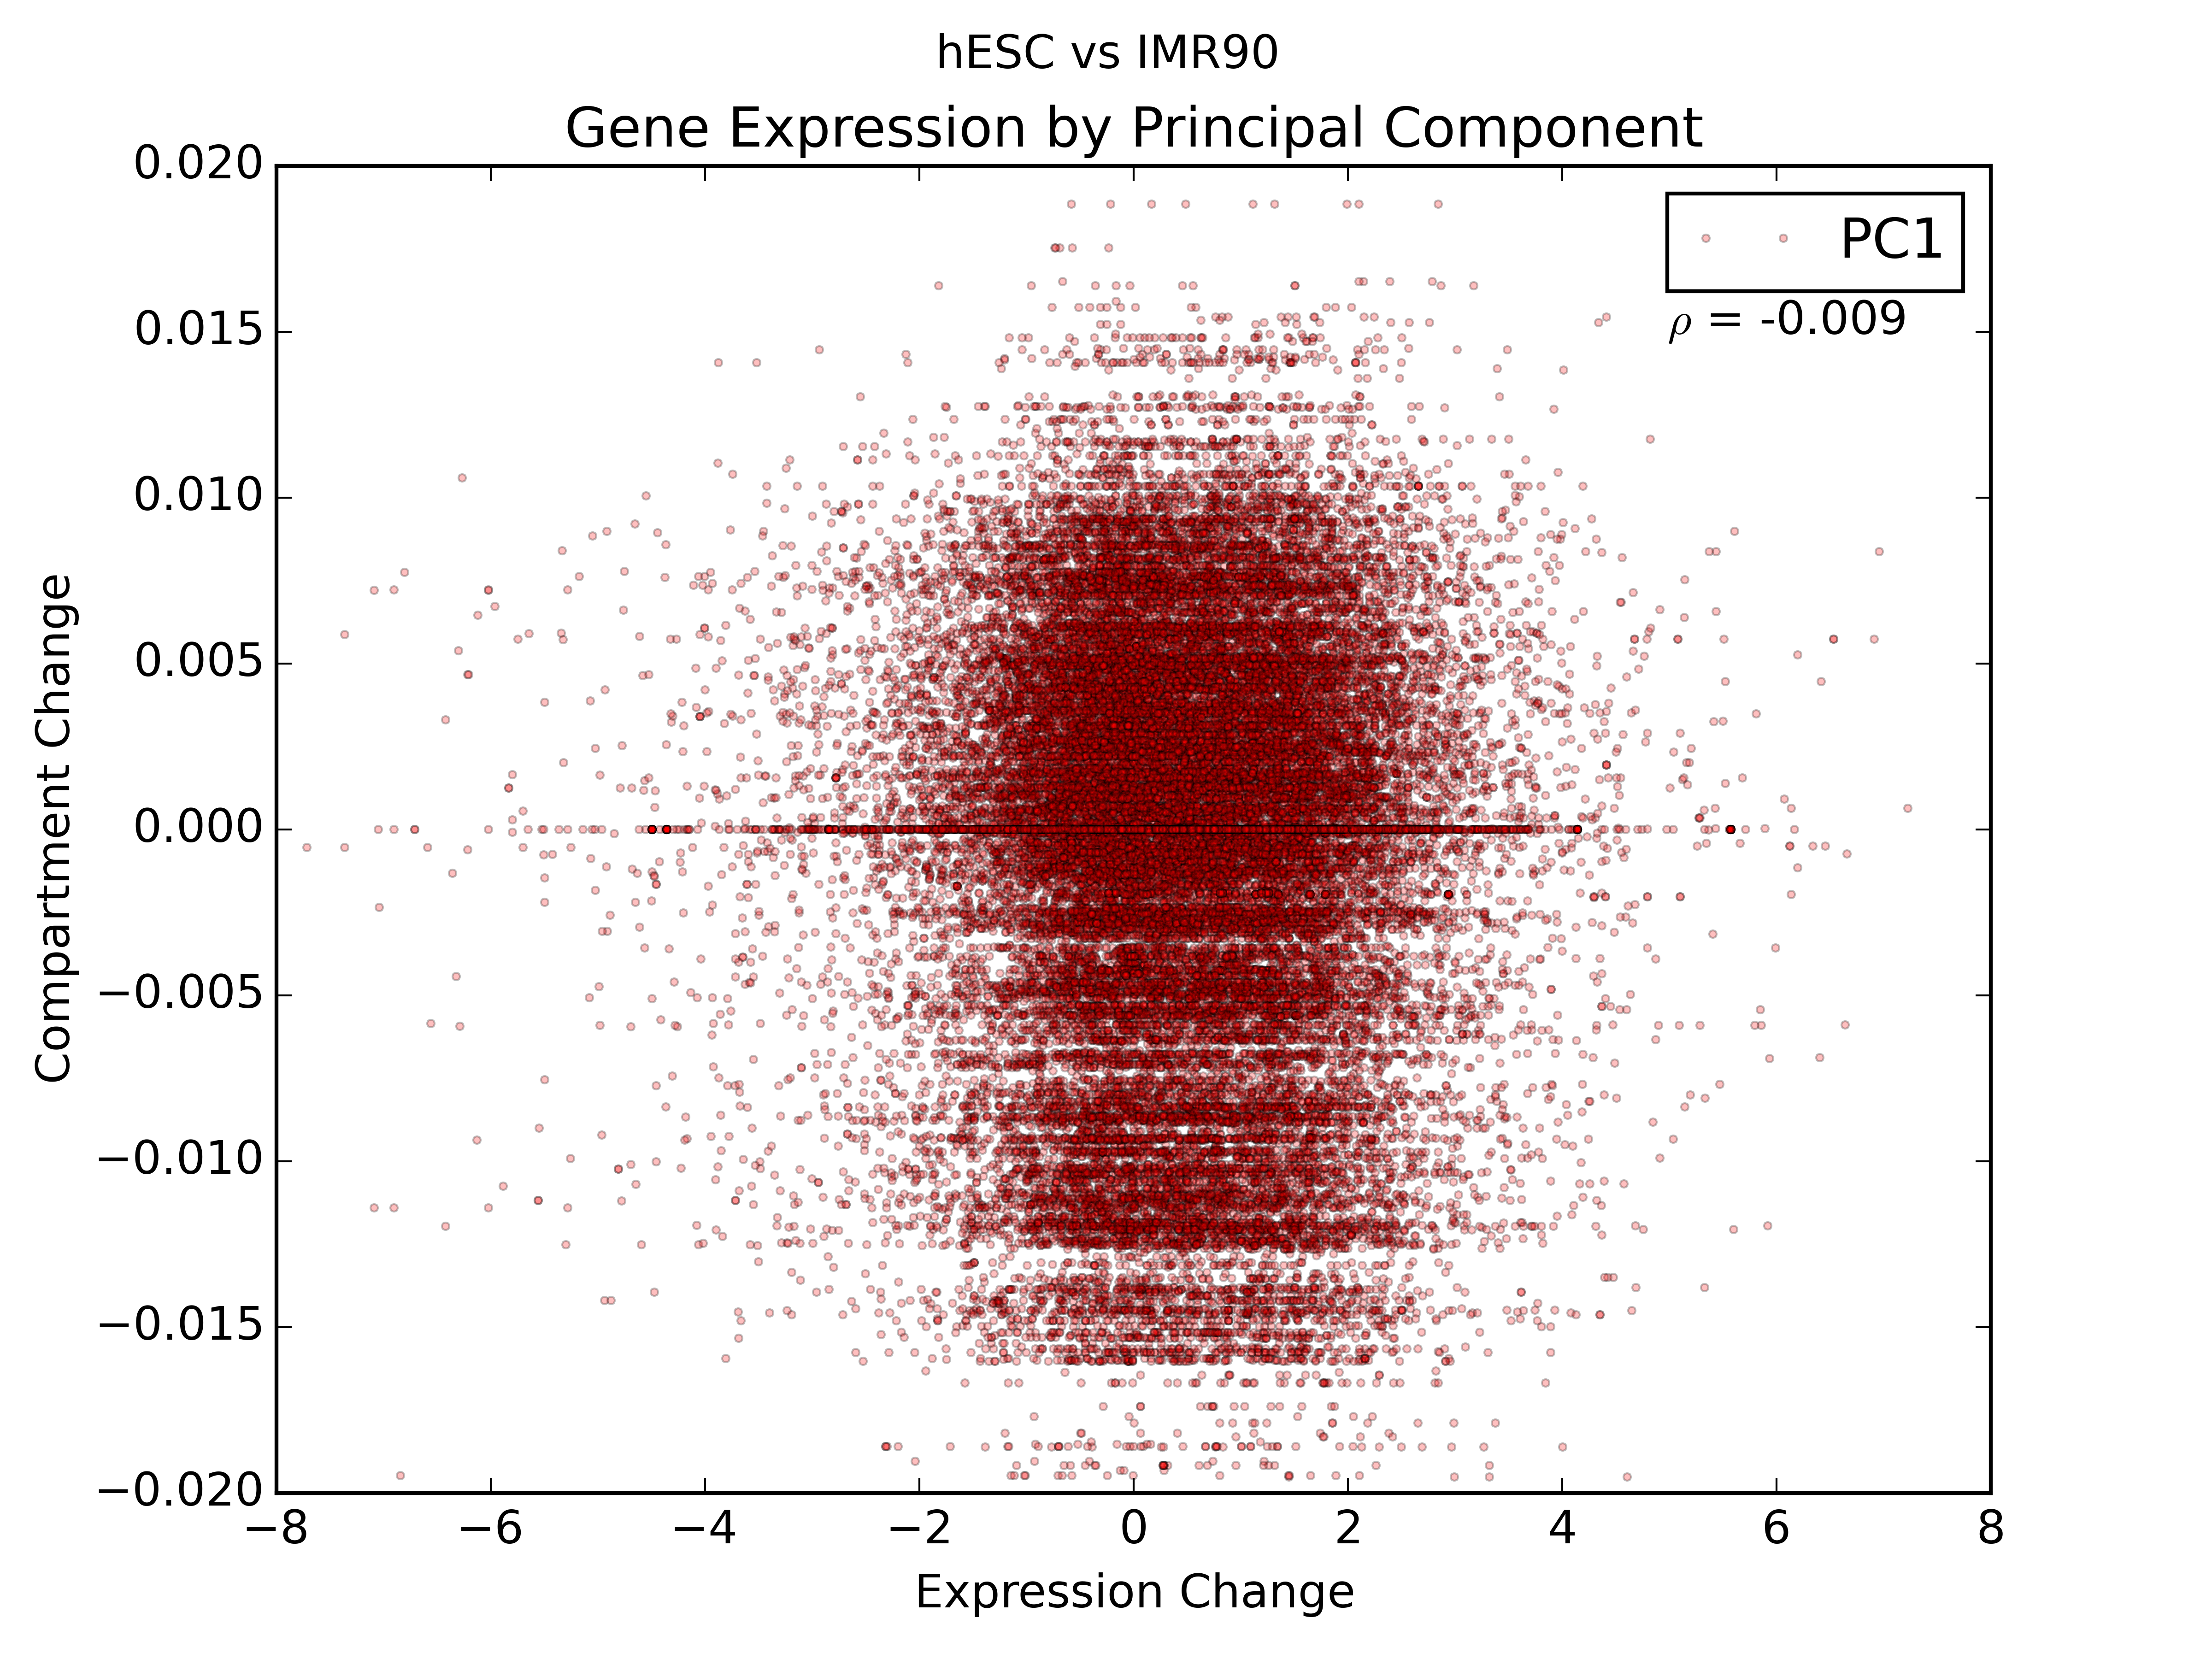
\includegraphics[width=\textwidth]{./figures/results/volcano.png}
  \end{minipage}

  \begin{minipage}{0.45\textwidth}
    \centering
    \caption{Compartmentalized Gene Expression}\label{fig:expressionChangeByCompartment}
    \includegraphics[width=\textwidth]{./figures/results/compartment_ir5_200k.png}
  \end{minipage}
\end{figure}

\section*{Eigenvector Partitioning}

The original Hi-C experiment revealed that the genome can be compartmentalized by \gls{PC} into two characteristic classes, arbitrarily
labeled A and B.  Lieberman-Aiden and colleagues showed positive correlations between compartment identity, gene density, and chromatin
accessibility, concluding that compartment A consists of largely open chromatin, while compartment B is densely packed \citep{aiden2009}.
Interestingly, we did not observe any correlation between the eigenvector and gene expression data (via genome-wide mRNA expression,
Spearman's $\rho = -0.014$, p negligible; Supplementary Information~\ref{}).  Furthermore, shifts in compartment character did not correlate to
changes in gene expression level (Spearman's $\rho = -0.01$, p negligible).  Given these results, it seems unlikely that cells regulate
gene expression at the compartment level.  Compartmentalization appears to be part of the larger nuclear architectural scheme, rather than
a dynamic regulatory mechanism.

Given the known differences between nuclear compartments, we investigated whether common fragile sites were clustered in a particular
compartment, conferring a level of fragility.

\begin{figure}[thp]
  \centering
  \caption{Fragile Sites in Compartments}\label{fig:compartmentCfs}
  \includegraphics[width=\textwidth]{./figures/results/cfs.png}
\end{figure}

\section*{Directionality Indices}

If the nuclear architecture can be decomposed into layers as we have hypothesized, topological domains may exist at different
scales or resolutions within the nucleus.  We tested this hypothesis by calculating directionality indices at various window sizes
on a high resolution contact map.  Interestingly, we found that the minimum correlations between indices at a given window size increased
with higher resolution map ($\rho_{\min}(100kb) = 0.77, \rho_{\min}(1Mb) = 0.70$, Supplementary Information~\ref{sec:SuppDirectionality}).

\section*{Domain Discovery}

Topological domains represent a novel level of genomic regulation.  Previous discovered domains show enrichment in chromatin modeling proteins,
housekeeping genes, and retrotransposons at the topological domain boundaries \citep{dixon2012}.  We used a naive heuristic to discover conserved
topological domain sets at smaller resolutions than previously reported.

\begin{figure}[thp]
  \caption{Number of Domains by Chromosome}
  \begin{minipage}{0.5\textwidth}%
    \centering
    \includegraphics[width=\textwidth]{./figures/results/domain_imr90_bar.png}
  \end{minipage}

  \begin{minipage}{0.5\textwidth}
    \centering
    \includegraphics[width=\textwidth]{./figures/results/domain_hesc_bar.png}
  \end{minipage}
\end{figure}

